%%%%%%%%%%%%%%%%%%%%%%%%%%%%%%%%%%%%%%%%%%%%%%%%%%%%%%%%%%%%%%%%%%%%%%%%
%                                                                      %
% This program is free software; you can redistribute it and/or modify %
% it under the terms of the GNU General Public License as published by %
% the Free Software Foundation; either version 2 of the License, or    %
% (at your option) any later version.                                  %
%                                                                      %
% This program is distributed in the hope that it will be useful,      %
% but WITHOUT ANY WARRANTY; without even the implied warranty of       %
% MERCHANTABILITY or FITNESS FOR A PARTICULAR PURPOSE.  See the        %
% GNU General Public License for more details.                         %
%                                                                      %
% You should have received a copy of the GNU General Public License    %
% along with this program; if not, write to the Free Software          %
% Foundation, Inc., 51 Franklin St, Fifth Floor, Boston,               %
% MA  02110-1301  USA                                                  %
%                                                                      %
%%%%%%%%%%%%%%%%%%%%%%%%%%%%%%%%%%%%%%%%%%%%%%%%%%%%%%%%%%%%%%%%%%%%%%%%
%
%	$Id$
%

\setcounter{remarque-cnt}{1}
\setcounter{example-cnt}{1}
\chapter{Commandes usuelles de communication r{\'e}seau}
\thispagestyle{fancy}

%%%%%%%%%%%%%%%%%%%%%%%%%%%%%%%%%%%%%%%%%%%%%%%%%%%%
\section{Connexion {\`a} une autre machine -- commande {\tt telnet}}

\begin{definition}{Syntaxe}
\begin{verbatim}
telnet [host [port]]
\end{verbatim}
\end{definition}

La commande \index{telnet@\texttt{telnet}}<<~{\tt telnet}~>> permet de communiquer avec une autre machine en utilisant le protocole {\sl Telnet}. Si <<~{\tt telnet}~>> est invoqu{\'e} sans argument, il passe en mode commande, indiqu{\'e} par l'invite <<~\verb=telnet>=~>>. Dans ce mode, il accepte et ex{\'e}cute des commandes. Si <<~{\tt telnet}~>> est invoqu{\'e} avec des arguments, il ouvre une connexion sur ce qui lui a {\'e}t{\'e} sp{\'e}cifi{\'e}.

Une fois qu'une connexion a {\'e}t{\'e} ouverte, <<~{\tt telnet}~>> passe en mode saisie. Dans ce mode, le texte tap{\'e} au clavier est envoy{\'e} {\`a} la machine cible.

Voici quelques \index{telnet@\texttt{telnet}!commandes internes {\`a}}commandes accessibles au niveau du prompt <<~\verb=telnet>=~>>~:

\begin{description}
	\item[{\tt open [host [port]]}]\mbox{}\\
		Ouvre une connexion sur le n{\oe}ud sp{\'e}cifi{\'e} au port indiqu{\'e}. Si aucun
		port n'est sp{\'e}cifi{\'e}, <<~{\tt telnet}~>> essaie de contacter un serveur
		{\sl Telnet} au port standard de {\sl Telnet}. Le nom de n{\oe}ud peut
		{\^e}tre soit le nom officiel, soit un {\sl alias}, soit une adresse Internet
		en notation d{\'e}cimale.
	\item[{\tt close}]\mbox{}\\
		Ferme une session <<~{\tt telnet}~>>. Si la session a commenc{\'e} en mode
		commande, alors <<~{\tt telnet}~>> repasse en mode commande; autrement,
		{\tt telnet} se termine.
	\item[{\tt ?}]\mbox{}\\
		Fournit de l'aide. Sans argument <<~{\tt ?}~>> affiche le menu d'aide. Si
		une commande est pr{\'e}cis{\'e}e apr{\`e}s <<~{\tt ?}~>>, le message affich{\'e}
		s'applique uniquement {\`a} la commande sp{\'e}cifi{\'e}e.
\end{description}

Pour plus d'informations, consultez {\tt telnet(1)}.

\begin{remarque}
<<~{\tt telnet}~>> est seulement un service interactif. Vous ne pouvez pas ex{\'e}cuter <<~{\tt telnet}~>> en arri{\`e}re-plan ou {\`a} partir d'un programme shell.
\end{remarque}

%%%%%%%%%%%%%%%%%%%%%%%%%%%%%%%%%%%%%%%%%%%%%%%%%%%%
\section{Transfert de fichiers - commande {\tt ftp}}

\begin{definition}{Syntaxe}
\begin{verbatim}
ftp [-g] [-i] [-n] [v] [host]
\end{verbatim}
\end{definition}

\index{ftp@\texttt{ftp}}<<~{\tt ftp}~>> est une famille de commandes pour les op{\'e}rations de manipulation de fichiers ou de r{\'e}pertoires {\`a} travers le r{\'e}seau.

Vous pouvez importer ou exporter des fichiers {\`a} partir d'une machine distante (sous {\Unix} ou non), en utilisant soit le mode de transfert
{\ASCII}, soit le mode de transfert {\sl binaire}.

Vous pouvez~:
\begin{itemize}
	\item mettre {\`a} jour, renommer et supprimer des fichiers,
	\item lister le contenu de r{\'e}pertoires,
	\item changer, cr{\'e}er et supprimer des r{\'e}pertoires,
	\item v{\'e}rifier l'{\'e}tat, changer les options,
	\item demander de l'aide.
\end{itemize}

<<~{\tt ftp}~>> admet quatre \index{ftp@\texttt{ftp}!options}options~:\\
\begin{tabular}{lc@{\hspace{2ex}}p{8cm}}
	{\tt -g}	& : &	inhibition des m{\'e}tacaract{\`e}res.\\
				&   &
		Lorsque cette option n'est pas pr{\'e}cis{\'e}e, par d{\'e}faut, les
		m{\'e}tacaract{\`e}res sont interpr{\'e}t{\'e}s pour l'importation ou l'exportation
		de fichiers. Pour plus de pr{\'e}cisions sur les m{\'e}tacaract{\`e}res,
		reportez vous {\`a} la section \ref{basic-metacars}.
		\\[0.5cm]
	{\tt -i}	& : &	inhibition du mode interactif sur les manipulations de
					fichiers.\\
				&   &
		Le mode interactif est actif par d{\'e}faut.
		\\[0.5cm]
	{\tt -n}	& : &	d{\'e}sactivation de la connexion automatique.\\
				&   &
		 La connexion automatique est autoris{\'e}e.
		\\[0.5cm]
	{\tt -v}	& : &	mode {\sl verbose}.\\
				&   &
		En l'absence de cette option, <<~{\tt ftp}~>> utilise le mode {\sl verbose}
		uniquement si la sortie standard est associ{\'e}e {\`a} un terminal.
		\\[0.5cm]
\end{tabular}

Quelques-unes des commandes de <<~{\tt ftp}~>> sont expliqu{\'e}es ci-dessous. Dans les explications, <<~{\tt server-host}~>> d{\'e}signe la machine sur laquelle on se connecte avec <<~{\tt ftp}~>>. <<~{\tt local-host}~>> d{\'e}signe la machine sur laquelle la commande <<~{\tt ftp}~>> a {\'e}t{\'e} lanc{\'e}e. La figure
\ref{fig-cmdnet-ftpdesc} illustre les terminologies utilis{\'e}es.

\begin{figure}[hbtp]
\centering
%\epsfbox{_Images/cmds-net/ftpdesc.eps}
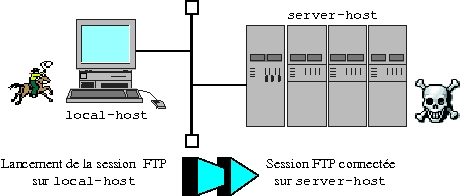
\includegraphics{cmds-net/ftpdesc}
\caption{\label{fig-cmdnet-ftpdesc}Terminologie pour la description de
		<<~{\tt ftp}~>>.}
\end{figure}

{\bf Apercu des \index{ftp@\texttt{ftp}!commandes internes {\`a}}commandes {\tt ftp}~:}\\
\begin{description}
	\item[{\tt open server-host [port-number]}]\mbox{}\\
	Etablit une connexion avec <<~{\tt server-host}~>> en utilisant un num{\'e}ro de port
	si sp{\'e}cifi{\'e}. Si aucun port n'est pr{\'e}cis{\'e}, <<~{\tt ftp}~>> essaie de
	contacter un serveur avec le num{\'e}ro de port standard.

	\item[{\tt user user\_name [password] [account]}]\mbox{}\\
	Connexion sous l'identit{\'e} <<~{\tt user\_name}~>> sur <<~{\tt
	server-host}~>> ouverte avec la commande <<~{\tt open}~>>. La figure
	\ref{fig-cmdnet-ftpconn} illustre l'{\'e}tablissement d'une connexion.
	\begin{figure}[hbtp]
	\centering
%	\epsfbox{_Images/cmds-net/ftpconn.eps}
	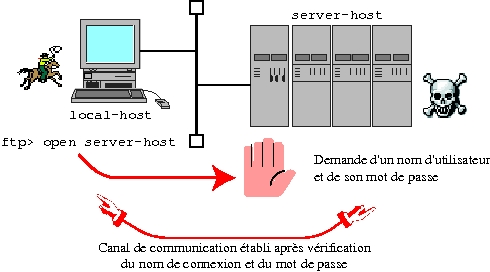
\includegraphics{cmds-net/ftpconn}
	\caption{\label{fig-cmdnet-ftpconn}Etablissement d'une connexion {\tt ftp}}
	\end{figure}

	\item[{\tt glob}]\mbox{}\\
	Autorise l'usage des m{\'e}tacaract{\`e}res. Si cette option est activ{\'e}e,
	<<~{\tt ftp}~>> envoie les m{\'e}tacaract{\`e}res {\`a} <<~{\tt server-host}~>> pour qu'il
	puisse les interpr{\'e}ter au niveau des noms de fichiers et des
	r{\'e}pertoires existants. La substitution des m{\'e}tacaract{\`e}res est
	toujours faite avec la commande <<~{\tt ls}~>>. Pour plus de pr{\'e}cisions
	sur les m{\'e}tacaract{\`e}res, preportez-vous {\`a} la section \ref{basic-metacars}.

	\item[{\tt binary}]\mbox{}\\
	Positionne l'option binaire pour le type de transfert de fichiers.

	\item[{\tt ls [remote\_dir [local\_file]]}]\mbox{}\\
	Affiche les noms des fichiers du site distant <<~{\tt remote\_dir}~>>
	{\`a} l'{\'e}cran, ou {\'e}ventuellement la redirige dans un fichier local
	<<~{\tt local\_file}~>>. Si <<~{\tt remote\_dir}~>> et <<~{\tt
	local\_file}~>> ne sont pas pr{\'e}cis{\'e}s,alors le r{\'e}pertoire de travail
	distant est affich{\'e} sur la sortie standard.


	\item[{\tt put local\_file [remote\_file]}]\mbox{}\\
	Copie un fichier local <<~{\tt local\_file}~>> vers le site distant
	sous le nom <<~{\tt remote\_file}~>>. Si <<~{\tt remote\_file}~>> n'est
	pas sp{\'e}cifi{\'e}, <<~{\tt ftp}~>> copie le fichier sous le m{\^e}me nom. La figure
	\ref{fig-cmdnet-ftpexch} illustre l'envoi et la r{\'e}ception de fichiers
	entre un serveur et un client <<~{\tt ftp}~>>.


	\item[{\tt mput local\_file local\_file ...}]\mbox{}\\
	Copie plusieurs fichiers du site local vers le site distant. Les
	fichiers de destination ont les m{\^e}mes noms que les fichiers locaux
	d'origine. Si l'option <<~{\tt glob}~>> est activ{\'e}e, les
	m{\'e}tacaract{\`e}res sont interpr{\'e}t{\'e}s. La figure \ref{fig-cmdnet-ftpexch}
	illustre l'envoi et la r{\'e}ception de fichiers entre un serveur et un
	client <<~{\tt ftp}~>>.


	\item[{\tt get remote\_file [local\_file]}]\mbox{}\\
	Copie un fichier distant <<~{\tt remote\_file}~>> sur le syst{\`e}me local
	sous le nom <<~{\tt local\_file}~>>. Si <<~{\tt local\_file}~>> n'est
	pas pr{\'e}cis{\'e}, <<~{\tt ftp}~>> copie le fichier avec le m{\^e}me nom. La figure
	\ref{fig-cmdnet-ftpexch} illustre l'envoi et la r{\'e}ception de fichiers
	entre un serveur et un client <<~{\tt ftp}~>>.


	\item[{\tt mget remote\_file remote\_file ...}]\mbox{}\\
	Copie plusieurs fichiers distants vers le syst{\`e}me local. Si l'option
	<<~{\tt glob}~>> est activ{\'e}e, les m{\'e}tacaract{\`e}res sont interpr{\'e}t{\'e}s. La figure
	\ref{fig-cmdnet-ftpexch} illustre l'envoi et la r{\'e}ception de fichiers
	entre un serveur et un client <<~{\tt ftp}~>>.

	\begin{figure}[hbtp]
	\centering
%	\epsfbox{_Images/cmds-net/ftpexch.eps}
	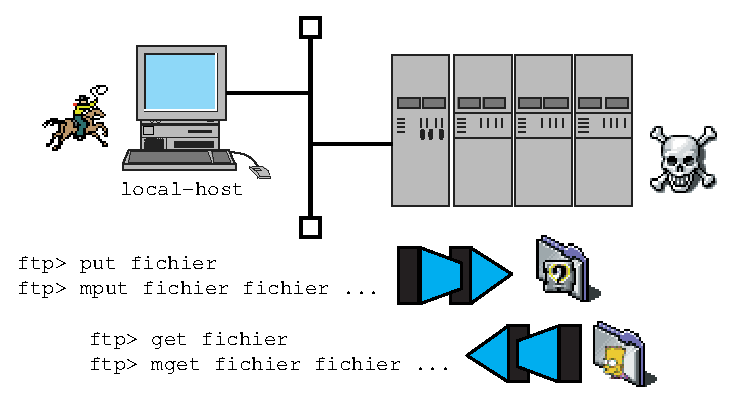
\includegraphics{cmds-net/ftpexch}
	\caption{\label{fig-cmdnet-ftpexch}Envoi/R{\'e}ception de fichier(s) de
	<<~{\tt server-host}~>> vers <<~{\tt local-host}~>> avec <<~{\tt ftp}~>>.}
	\end{figure}

	\item[{\tt close}]\mbox{}\\
	Ferme la connexion avec <<~{\tt server-host}~>>. La commande <<~{\tt
	close}~>> ne permet pas de sortir de <<~{\tt ftp}~>> si la connexion a {\'e}t{\'e}
	{\'e}tablie avec une commande <<~{\tt open}~>>.

	\item[{\sl {\tt quit} ou {\tt bye}}]\mbox{}\\
	Les commandes <<~{\tt quit}~>> et <<~{\tt bye}~>> ont le m{\^e}me effet.
	Elles ferment la connexion avec <<~{\tt server-host}~>> si une
	connexion {\'e}tait ouverte et sort de <<~{\tt ftp}~>>.
\end{description}

\begin{example}
{\bf Utilisation de <<~{\tt ftp}~>> dans un programme shell}
\begin{quote}
Vous pouvez utiliser <<~{\tt ftp}~>> dans un programme shell en respectant
certaines r{\`e}gles. Voici un exemple d'utilisation de <<~{\tt ftp}~>> dans un
programme Bourne Shell.

\begin{verbatim}
(
    for host in willow arthur merlin
    do
        echo "
            open $host
            user lancelot dulac
            binary
            mput excalibur*
            close
        "
    done
) | ftp -i -n
\end{verbatim}

Ce programme shell repr{\'e}sente un risque au niveau de la s{\'e}curit{\'e} (mot de passe en clair dans une proc{\'e}dure). Ce type de programme est {\`a} utiliser avec parcimonie. Pour plus de renseignements, consultez <<~{\tt ftp(1)}~>>.
\end{quote}
\end{example}

%%%%%%%%%%%%%%%%%%%%%%%%%%%%%%%%%%%%%%%%%%%%%%%%%%%%%%%
\section{Connexion automatique -- commande {\tt rlogin}}

\begin{definition}{Syntaxe}
{\tt rlogin remote\_host [-e{\it c}] [-l {\it username}]}
\end{definition}

La commande \index{rlogin@\texttt{rlogin}}<<~{\tt rlogin}~>> connecte votre terminal du site local sur un n{\oe}ud distant. <<~{\tt rlogin}~>> agit comme un terminal virtuel sur le syst{\`e}me distant. Le nom de machine distante peut {\^e}tre le nom officiel ou bien un {\sl alias}\footnote{Nom secondaire au niveau de la configuration r{\'e}seau.}. Il est possible aussi d'utiliser l'adresse Internet. Le type de terminal (indiqu{\'e} par la variable <<~{\tt TERM}~>>) est propag{\'e} {\`a} travers le r{\'e}seau et est utilis{\'e} pour initialiser la variable <<~{\tt TERM}~>> sur le site distant. Pour plus de renseignements sur les variables d'environnement du shell, reportez vous {\`a} la section \ref{basicn-codevar}.

Une fois connect{\'e} au site distant, vous pouvez ex{\'e}cuter des commandes sur le site local en utilisant le caract{\`e}re d'{\'e}chapement (par d{\'e}faut <<~{\verb=~=}~>>). Une ligne commen\c{c}ant par <<~\verb=~!=~>> cr{\'e}e un shell et vous permet d'ex{\'e}cuter temporairement des commandes sur le site local. Une ligne commen\c{c}ant par <<~\verb=~=~>> vous d{\'e}connecte du site distant. Plus simplement, pour revenir {\`a} votre session de d{\'e}part, il suffit de taper la commande <<~{\tt exit}~>> sur le site distant.

\begin{example}
\verb=dragon % rlogin king -l arthur=\\
\verb=Password:=\\
\verb=Welcome on IRIX 4.5 4D/480 to node king=\\
\verb=king% ~!=\\
\verb=dragon %=\hfill \hfill (vous {\^e}tes de retour sur votre terminal local)\\
$\cdots$\\
\verb=dragon % exit=\hfill \hfill(vous retournez {\`a} la station distante)\\
\verb=king%=
\end{example}

Les options de rlogin sont d{\'e}crites ci-dessous~:\\[0.5ex]
\begin{tabular}{lp{8cm}}
	{\tt -e{\it c}}		&
	Positionne le caract{\`e}re d'{\'e}chappement {\`a} <<~{\tt c}~>>. Il n'y a pas d'espace
	entre le caract{\`e}re <<~{\tt e}~>> et le caract{\`e}re d'{\'e}chappement.\\
	{\tt -l {\it username}}	&
	Met le nom de connexion de l'utilisateur sur le site distant {\`a} <<~{\tt
	username}~>>. Par d{\'e}faut, le nom de connexion de l'utilisateur sur le
	site local est utilis{\'e} pour se connecter au site distant.
\end{tabular}

Pour plus de renseigements, consultez <<~{\tt rlogin(1)}~>>.

%%%%%%%%%%%%%%%%%%%%%%%%%%%%%%%%%%%%%%%%%%%%%%%%%%%%%%%
\section{Transfert de fichiers automatique -- commande {\tt rcp}}

\begin{definition}{Syntaxe}
{\tt rcp {\it source} {\it destination}}

avec {\it source} et {\it destination} de la forme {\tt [[{\it user}@]{\it host}:]{\it pathname}}
\end{definition}

La commande \index{rcp@\texttt{rcp}}<<~{\tt rcp}~>> est similaire {\`a} la commane <<~{\tt cp}~>> d'{\Unix}. Comme <<~{\tt cp}~>>, <<~{\tt rcp}~>> aura un comportement diff{\'e}rent selon le nombre d'arguments~:

\begin{itemize}
	\item	si elle ne poss{\`e}de que deux arguments, elle copie le fichier source
			sous le nouveau nom,
	\item	si elle poss{\`e}de plusieurs arguments, la destination est
			obligatoirement un r{\'e}pertoire. Dans ce cas, elle copie les fichiers
			sources dans le r{\'e}pertoire sp{\'e}cifi{\'e}.
\end{itemize}

<<~{\tt rcp}~>> ne demande pas de mot de passe si une {\'e}quivalence syst{\`e}me ou utilisateur a {\'e}t{\'e} configur{\'e}e.

Dans le cas contraire, elle ne fonctionne pas (message <<~{\tt Permission denied}~>>). <<~{\tt rcp}~>> autorise des transferts mettant en jeu plusieurs machines. Par exemple, si vous {\^e}tes connect{\'e} sur une machine, vous pouvez transf{\'e}rer des fichiers entre deux n{\oe}uds du r{\'e}seau totalement diff{\'e}rents.

La source et la destination se pr{\'e}sentent sous la forme
{\tt [[{\it user}@]{\it host}:]{\it pathname}} avec~:\\
\begin{center}
\begin{tabular}{lp{8cm}}
	{\tt host}		&
	Sp{\'e}cifie le syst{\`e}me sur lequel se trouve le fichier. Si <<~{\tt
	host}~>> n'est pas pr{\'e}cis{\'e}, le syst{\`e}me local est utilis{\'e} par d{\'e}faut.\\
	{\tt user}		&
	Sp{\'e}cifie l'utilisateur sur <<~{\tt host}~>>. Si <<~{\tt user}~>> n'est
	pas pr{\'e}cis{\'e}, l'utilisateur sur le site distant est le m{\^e}me que sur
	le site local (les noms des utilisateurs doivent correspondre d'un
	syst{\`e}me {\`a} l'autre).\\
	{\tt pathname}	&
	Donne le chemin du fichier {\`a} copier. Il peut {\^e}tre relatif ou absolu.
	Un chemin relatif est interpr{\'e}t{\'e} de mani{\`e}re relative par rapport au
	r{\'e}pertoire de connexion sur le site distant ou par rapport au
	r{\'e}pertoire courant sur le site local.
\end{tabular}
\end{center}

Il est possible d'utiliser les m{\'e}tacaract{\`e}res pour r{\'e}f{\'e}rencer des fichiers. N'oubliez pas que le shell local interpr{\`e}te n'importe quel m{\'e}tacaract{\`e}re avant d'appeler <<~{\tt rcp}~>>. Pour emp{\^e}cher une substitution locale des m{\'e}tacaract{\`e}res devant {\^e}tre trait{\'e}s par le site distant, mettez les entre simples quotes (cf. section \ref{basic-quotes}).

\begin{example}
\label{exp-cmdnet-exrcp}
On supposera que toutes les {\'e}quivalences utilisateur et syst{\`e}me ont {\'e}t{\'e} configur{\'e}es correctement.

Le processus de cet exemple est d{\'e}crit au tableau \ref{tab-cmdnet-exrcp} et {\`a} la figure \ref{fig-cmdnet-exrcp}.
\end{example}

Dans la configuration d{\'e}crite dans la figure \ref{fig-cmdnet-exrcp},\\
\begin{longtable}{|c|p{8cm}|}
	\hline
	\multicolumn{2}{|r|}{Suite de la page pr{\'e}c{\'e}dente.} \\
	\hline
	\multicolumn{1}{|c|}{Exemple}		&
	\multicolumn{1}{|c|}{Description}	\\
	\hline
\endhead
	\hline
	\multicolumn{1}{|c|}{Exemple}		&
	\multicolumn{1}{|c|}{Description}	\\
	\hline
\endfirsthead
	\hline
		\multicolumn{2}{|r|}{Suite page suivante $\cdots$} \\
	\hline
\endfoot
	\hline
\endlastfoot
	\hline
 	\raisebox{-0.5cm}{
%\epsfbox{_Images/cmds-net/exrcp-cl1.eps}

\includegraphics{cmds-net/exrcp-cl1}
}	&
	L'utilisateur {\tt willow} sur la machine {\tt dragon} copie le
	fichier {\tt excalibur.c} de l'utilisateur {\tt arthur} sur la
	machine {\tt king} dans son r{\'e}pertoire courant.
	\\
	\hline
  	\raisebox{-0.5cm}{
%\epsfbox{_Images/cmds-net/exrcp-cl2.eps}

\includegraphics{cmds-net/exrcp-cl2}
}	&
	L'utilisateur {\tt willow} sur la machine {\tt dragon} copie le
	fichier local {\tt donjon.c} sur la machine {\tt dragon} vers le
	r{\'e}pertoire de connexion de l'utilisateur {\tt willow} sur la machine
	{\tt dulac}.
	\\
	\hline
 	\raisebox{-0.5cm}{
%\epsfbox{_Images/cmds-net/exrcp-cl3.eps}

\includegraphics{cmds-net/exrcp-cl3}
}	&
	L'utilisateur {\tt willow} sur la machine {\tt dragon} copie tous les
	fichiers <<~{\tt .c}~>> de l'utilisateur {\tt arthur} sur la machine
	{\tt king} vers son r{\'e}pertoire courant.
	\\
	\hline
 	\raisebox{-0.5cm}{
%\epsfbox{_Images/cmds-net/exrcp-cl4.eps}
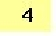
\includegraphics{cmds-net/exrcp-cl4}
}	&
	L'utilisateur {\tt willow} sur la machine {\tt dragon} copie le
	fichier {\tt excalibur.c} de l'utilisateur {\tt arthur} sur la
	machine {\tt king} vers le r{\'e}pertoire de connexion de l'utilisateur
	{\tt lancelot} sur la machine {\tt dulac}.
	\\
	\hline
\caption*{\label{tab-cmdnet-exrcp}Description des op{\'e}rations effectu{\'e}es.}
\end{longtable}

On obtient l'exemple illustr{\'e} dans la figure \ref{fig-cmdnet-exrcp}.

\begin{figure}
\centering
%\epsfbox{_Images/cmds-net/exrcp.eps}
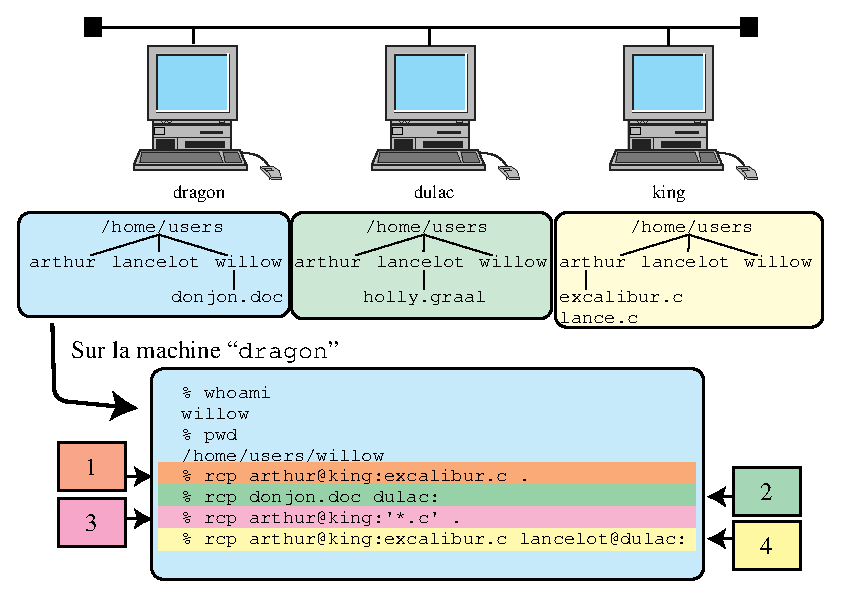
\includegraphics{cmds-net/exrcp}
\caption{\label{fig-cmdnet-exrcp}Exemple d'utilisation de la commande <<~{\tt rcp}~>>.}
\end{figure}


%%%%%%%%%%%%%%%%%%%%%%%%%%%%%%%%%%%%%%%%%%%%%%%%%%%%%%%
\section{Ex{\'e}cution d'une commande {\`a} distance - commande {\tt rsh} (ou {\tt remsh})}

\begin{definition}{Syntaxe}
{\tt rsh [-l {\it username}] [-n] {\it commande}}\\
{\tt remsh [-l {\it username}] [-n] {\it commande}}
\end{definition}

Les commandes \index{rsh@\texttt{rsh}}<<~\texttt{rsh}~>> et \index{remsh@\texttt{remsh}}<<~\texttt{remsh}~>> sont {\'e}quivalentes.
Sur certains syt{\`e}mes il n'exite que la commande <<~\texttt{rsh}~>>\footnote{\textsl{SunOS} et  \textsl{Solaris} sur les syst{\`e}mes de Sun Microsystems, \textsl{Irix} sur les machines de Silicon Graphics, \textsl{Digital {\Unix}} sur les machines de Compacq - ex Digital Equipment Corp.}, sur d'autres que seule la commande <<~{\tt remsh}~>> sera disponible\footnote{\textsl{UTekV} sur les anciens syst{\`e}mes {\Unix} de Tektronix, \textsf{HP--UX} sur les syst{\`e}mes de Hewlett-Packard}), sur d'autres les deux cohabiteront\footnote{AIX, l'{\Unix} d'IBM}. Dans toute la suite de ce paragraphe, seulement <<~\texttt{rsh}~>> sera cit{\'e}.

La commande <<~{\tt rsh}~>> ex{\'e}cute une commande non interactive sur un syst{\`e}me distant. Le nom du compte est le m{\^e}me que le nom du compte local {\`a} moins que vous ne sp{\'e}cifiez l'option <<~{\tt -l}~>>.

Comme <<~{\tt rcp}~>>, <<~{\tt rsh}~>> ne demande pas de mot de passe si une {\'e}quivalence syst{\`e}me ou utilisateur a {\'e}t{\'e} configur{\'e}e. Dans le cas contraire, elle ne fonctionne pas (message <<~{\tt Permission denied}~>>). La commande <<~{\tt rsh}~>> transmet les signaux <<~{\tt INTERRUPT}~>>, <<~{\tt QUIT}~>> et <<~{\tt HUP}~>> {\`a} la commande distante.

Pour plus de pr{\'e}cisions, reportez vous {\`a} <<~{\tt signal(2)}~>> et au chapitre \ref{multitask}.

Vous pouvez utiliser les m{\'e}tacaract{\`e}res avec <<~{\tt rsh}~>>. Si vous voulez qu'ils soient interpr{\'e}t{\'e}s sur le site distant, assurez-vous qu'ils sont bien entre simples quotes (cf. sections \ref{basic-metacars} et \ref{basic-quotes}).

\begin{remarque}
<<~{\tt rsh}~>> ne peut pas ex{\'e}cuter des commandes en mode interactif comme
<<~{\tt vi}~>>, <<~{\tt emacs}~>>, etc.
\end{remarque}

%%%%%%%%%%%%%%%%%%%%%%%%%%%%%%%%%%%%%%%%%%%%%%%%%%%%
\section{Connexion chiffr{\'e}e {\`a} une autre machine -- commande {\tt ssh}}
Les commandes pr{\'e}c{\'e}dentes ont non seulement des limitations (<<~{\tt rsh}~>> ne permet, par exemple, d'ex{\'e}cuter des commandes interactives) mais posent aussi des probl{\`e}mes de s{\'e}curit{\'e}. D{\'e}sormais, le protocole \index{ssh@\texttt{ssh}}<<~\texttt{ssh}~>> (\href{http://fr.wikipedia.org/wiki/Secure_shell/}{Secure SHell}), et la commande qui lui est associ{\'e}, est donc aujourd'hui le plus souvent utilis{\'e}, {\`a} la place de rlogin ou rsh .
Caract{\'e}ristique important, le protocole impose, au d{\'e}but de la communication, l'{\'e}change de cl{\'e} de cryptage, permettant au reste de la dialogue de s'effectuer de mani{\`e}re chiffr{\'e}.
L'implementation de <<~{\tt ssh}~>> la plus courament utilis{\'e} est celle du projet libre \href{http://www.openssh.org/fr/index.html}{OpenSSH}.
\begin{definition}{Syntaxe}
\begin{verbatim}
ssh [user]@[host:[port]]
\end{verbatim}
\end{definition}
Un rapide exemple de connexion sur une machine distante {\`a} l'aide de ssh:
\begin{verbatim}
ssh -l arthur percival -p 22
\end{verbatim}

La syntaxe suivante, plus explicite, est aussi possible:
\begin{verbatim}
ssh arthur@percival:22 
\end{verbatim}


\begin{remarque}
Le client <<~{ssh}~>> est un outil extremement puissant, qui permet, entre autres l'{\'e}tablissement de tunnel chiffr{\'e}, {\`a} travers plusieurs machines. N'h{\'e}sitez pas {\`a} en explorer les capacit{\'e}s. L'article \href{http://www.unixgarden.com/index.php/administration-systeme/principes-et-utilisation-de-ssh}{principe et utilisation de SSH} vous permettra d'aller plus loin.
\end{remarque}
% 
\begin{remarque}
Le client <<~{ssh}~>> peut tre utilis{\'e} comme un filtre, mais de mani{\`e}re assez particuli{\`e}re. Un rapide exemple pour illuster ce point:
\begin{verbatim}
cat mon\_fichier | ssh percival ``cat > mon\_fichier\_distant'' 
\end{verbatim}

La commande local cat va transf{\'e}rer vers ssh le contenu du mon\_fichier, ce dernier va le mettre {\`a} disposition sur le flux d'entr{\'e} du serveur distant (percival). Sur ce dernier, la commande cat va permettre de rediriger le flux vers mon\_fichier\_distant. 
\end{remarque}

\section{Transfert chiffr{\'e}e de fichier -- commande scp}
La commande  \index{scp@\texttt{scp}}<<~\texttt{scp}~>> permet d'utiliser le protocole ssh pour transf{\'e}rer des fichiers, mais dans un flux chiffr{\'e}. 

Attention, il est important (et {\'e}vident) de retenir que tout {\'e}change de fichier par ssh sera plus long et plus consommateur de resources du syst{\`e}me qu'un simple transfert en clair.
\begin{definition}{Syntaxe}
\begin{verbatim}
scp [user]@[host:[port]]file [user]@[host:[port]]fichier 
\end{verbatim}
\end{definition}



\subsection{Comparaisons \texttt{telnet}/\texttt{rlogin}/\texttt{ssh} et \texttt{ftp}/\texttt{rcp}/\texttt{scp}}

\index{telnet@\texttt{telnet}!comparaison avec \texttt{rlogin} et \texttt{ssh}}
\index{ssh@\texttt{ssh}!comparaison avec \texttt{rlogin} et \texttt{telnet}}
\index{rlogin@\texttt{rlogin}!comparaison avec \texttt{telnet}}
\begin{longtable}{|p{6.5cm}|p{2cm}|p{2cm}|p{2cm}|}
	\hline
		\multicolumn{4}{|r|}{Suite de la page pr{\'e}c{\'e}dente.} \\
	\hline
		\multicolumn{1}{|c|}{Fonctionnalit{\'e}}	&
		\multicolumn{1}{|c|}{{\tt telnet}}	&
		\multicolumn{1}{|c|}{rlogin}	&
		\multicolumn{1}{|c|}{ssh}	\\
	\hline
\endhead
	\hline
		\multicolumn{1}{|c|}{Fonctionnalit{\'e}}	&
		\multicolumn{1}{|c|}{{\tt telnet}}	&
		\multicolumn{1}{|c|}{rlogin}	&
		\multicolumn{1}{|c|}{ssh}	\\
	\hline \hline
\endfirsthead
	\hline
		\multicolumn{4}{|r|}{Suite page suivante $\cdots$} \\
	\hline
\endfoot
	\hline
\endlastfoot
	\hline
		Ensemble de commandes.		&
		Oui				&
		Non				&
		Oui				\\
	\hline
		Peut se connecter {\`a} des syst{\`e}mes non {\Unix}.	&
		Oui								&
		Non\footnote{D{\'e}pend de l'implantation sur le syst{\`e}me non-{\Unix}.}	&
		Oui\footnote{Si le syst{\`e} h{\^o}te dispose d'un serveur SSH, ce qui est g{\'e}n{\'e}ralement le cas. Pour indication, OpenSSH fonctionne sur Windows et OpenVMS.} \\
	\hline
		Peut {\^e}tre configur{\'e} en connexion automatique.	&
		Non								&
		Oui (fichiers {\tt /etc/hosts.equiv} et {\tt \~/.rhosts})	&
		Oui(Utilisation de cl{\'e} priv{\'e}e)	\\
	\hline
		Peut utiliser l'adresse IP pour la connexion.	&
		Oui								&
		Oui								&
		Non								\\
	\hline
		Sortie autoris{\'e}e.				&
		Oui (vers <<~{\tt telnet}~>> en mode commande)	&
		Oui (vers le terminal local)			&
		Oui						\\
	\hline
		Nombre de modes.				&
		2 (commande et connect{\'e})			&
		1 (connect{\'e} seulement)			&
		1 (connection partageable\footnote{Avec l'option -o ControlMaster})	\\
	\hline
		Peut {\^e}tre lac{\'e} depuis un programme Shell.	&
		Non													&
		Non													&
		Oui													\\
	\hline
\caption{Comparaisons {\tt telnet}/{\tt rlogin}/{\tt ssh}} \\
\end{longtable}

\begin{remarque}
Notez que <<~{\tt telnet}~>> et <<~{\tt rlogin}~>> peuvent {\^e}tre appel{\'e}s
depuis un programme Shell, mais vous ne pouvez pas leur transmettre des
informations au clavier (comme vous pouvez le faire avec <<~{\tt ftp}~>>).
\end{remarque}

\index{ftp@\texttt{ftp}!comparaison avec \texttt{rcp} et \texttt{scp}}
\index{rcp@\texttt{rcp}!comparaison avec \texttt{ftp} et \texttt{scp}}
\index{scp@\texttt{scp}!comparaison avec \texttt{ftp} et \texttt{rcp}}
\begin{longtable}{|p{6.5cm}|p{2cm}|p{2cm}|p{2cm}|}
	\hline
		\multicolumn{4}{|r|}{Suite de la page pr{\'e}c{\'e}dente.} \\
	\hline
		\multicolumn{1}{|c|}{Fonctionnalit{\'e}}	&
		\multicolumn{1}{|c|}{{\tt ftp}}			&
		\multicolumn{1}{|c|}{{\tt rcp}}			&
		\multicolumn{1}{|c|}{{\tt scp}}		\\
	\hline
\endhead
	\hline
		\multicolumn{1}{|c|}{Fonctionnalit{\'e}}	&
		\multicolumn{1}{|c|}{{\tt ftp}}			&
		\multicolumn{1}{|c|}{{\tt rcp}}			&
		\multicolumn{1}{|c|}{{\tt scp}}		\\
	\hline \hline
\endfirsthead
	\hline
		\multicolumn{4}{|r|}{Suite page suivante $\cdots$} \\
	\hline
\endfoot
	\hline
\endlastfoot
	\hline
		Ensemble de commandes	&
		Oui						&
		Non						&
		Oui						\\
	\hline
		Peut transf{\'e}rer des fichiers sur un syst{\`e}me non {\Unix}	&
		Oui						&
		Non\footnote{Sauf impl{\'e}mentation d'un serveur supportant
		ce type de connexion.}				&
		Non\footnote{Sauf impl{\'e}mentation d'un serveur supportant
		ce type de connexion.}				\\
	\hline
		Peut {\^e}tre ex{\'e}cut{\'e} dans un programme Shell	&
		Oui						&
		Oui						&
		Oui						\\
	\hline
		Peut mettre en jeu 3 n{\oe}uds	&
		Non		&
		Oui		&
		Oui		\\
	\hline
		Autorise les m{\'e}tacaract{\`e}res	&
		Oui (commande <<~{\tt glob}~>>)		&
		Oui					&
		Non					\\
	\hline
		Peut faire une copie r{\'e}cursive	&
		Non					&
		Oui (option <<~{\tt -r}~>>)		&
		Oui (option <<~{\tt -r}~>>)		\\
	\hline
		Peut configurer une {\'e}quivalence utilisateur				&
		Oui (fichier <<~{\tt \~/.netrc}~>>)					&
		Oui (fichiers <<~{\tt /etc/hosts.equiv}~>>, <<~{\tt \~/.rhosts}~>>)	&
		Oui (cl{\'e} priv{\'e}e)	\\
	\hline
		Equivalence utilisateur requise		&
		Non					&
		Oui					&
		Oui					\\
	\hline
		Peut utiliser une adresse IP pour la connexion	&
		Oui		&
		Oui		&
		Non		\\
	\hline
\caption{Comparaisons {\tt ftp}/{\tt rlogin}/{\tt scp}} \\
\end{longtable}
